\makeatletter
\let\pd@OrigRequirePackage\RequirePackage
\def\pd@dvipsname{dvips}
\def\RequirePackage{\@ifnextchar[\pd@RP@i{\pd@RP@i[\@empty]}}
\def\pd@RP@i[#1]#2{\@ifnextchar[{\pd@RP@ii{#1}{#2}}{\pd@RP@ii{#1}{#2}[\@empty]}}
\def\pd@RP@ii#1#2[#3]{%
  \def\pd@rpname{#2}%
  \ifx\pd@rpname\pd@hyperrefname
    \def\pd@newopts{}%
    \def\pd@first{1}%
    \ifx#1\@empty\else
      \@for\pd@tempopt:=#1\do{%
        \ifx\pd@tempopt\pd@dvipsname\else
          \ifx\pd@first\@empty
            \edef\pd@newopts{\pd@newopts,\pd@tempopt}%
          \else
            \edef\pd@newopts{\pd@tempopt}%
            \def\pd@first{}%
          \fi
        \fi
      }%
    \fi
    \ifx#3\@empty
      \pd@OrigRequirePackage[\pd@newopts]{#2}%
    \else
      \pd@OrigRequirePackage[\pd@newopts]{#2}[#3]%
    \fi
  \else
    \ifx#3\@empty
      \pd@OrigRequirePackage[#1]{#2}%
    \else
      \pd@OrigRequirePackage[#1]{#2}[#3]%
    \fi
  \fi
}
\def\pd@hyperrefname{hyperref}
\def\c@lor@to@ps#1 #2\@@{}%
\def\pdfmark#1{}%
\makeatother
\documentclass[style=ciment]{powerdot}
\def\pdcontentsline#1#2#3{}
\makeatletter
\def\pd@title#1{\begin{center}#1\end{center}}
\makeatother
\pddefinetemplate[titleslide]{titleslide}{texthook=tl,textpos={.05\slidewidth,.7\slideheight},textwidth=.9\slidewidth}{}
\pddefinetemplate[slide]{slide}{textpos={.05\slidewidth,.76\slideheight},textheight=.6\slideheight}{}

\usepackage[T1]{fontenc}
\usepackage{lmodern}
\usepackage{colortbl}
\usepackage{booktabs}
\usepackage{array}
\usepackage{tabularx}
\usepackage{tikz}
\usetikzlibrary{positioning,calc,shapes.geometric,decorations.pathmorphing,backgrounds,arrows.meta}
\usepackage{tcolorbox}
\tcbuselibrary{skins}
\usepackage{fontawesome5}
\usepackage{graphicx}

\definecolor{merinavy}{RGB}{27,42,74}
\definecolor{meringold}{RGB}{201,162,75}
\definecolor{merislate}{RGB}{91,107,121}
\definecolor{merilight}{RGB}{232,236,242}

\AtBeginDocument{%
  \definecolor{pdcolor2}{RGB}{27,42,74}%
  \definecolor{pdcolor3}{RGB}{91,107,121}%
  \definecolor{pdcolor4}{RGB}{232,236,242}%
}

\tcbset{
  meribox/.style={
    colback=merilight,
    colframe=merinavy,
    boxrule=0.4pt,
    arc=2pt,
    left=6pt, right=6pt, top=5pt, bottom=5pt,
    fonttitle=\bfseries\color{white},
    coltitle=white,
    colbacktitle=merinavy,
    boxsep=1pt
  },
  statbox/.style={
    colback=white,
    colframe=merislate,
    boxrule=0.4pt,
    arc=1pt,
    left=6pt, right=6pt, top=6pt, bottom=6pt
  }
}

\newcommand{\sectiondivider}[2]{%
\begin{slide}{}
\vspace{1.6cm}
\begin{center}
{\Large\textsf{\textcolor{merislate}{#1}}}\\[0.5cm]
{\color{meringold}\rule{4.2cm}{1.6pt}}\\[0.6cm]
{\huge\textbf{\textcolor{merinavy}{#2}}}
\end{center}
\end{slide}}

\title{\textcolor{merinavy}{Meridian Group}\\[6pt]{\large\textcolor{merislate}{FY2027 Strategic Plan}}}
\author{Elena Whitfield\\{\small Chief Strategy Officer}}
\date{14 October 2026}

\begin{document}

\maketitle

\begin{slide}{Agenda}
\begin{enumerate}
  \item Market Landscape
  \item Strategic Priorities
  \item Financial Outlook
  \item Execution \& Governance
\end{enumerate}
\vspace{0.8cm}
{\small\textcolor{merislate}{This document is prepared for the Meridian Group Board of Directors and senior leadership. All figures are management estimates unless noted as audited.}}
\end{slide}

\sectiondivider{SECTION 01}{Market Landscape}

\begin{slide}{Global Market Momentum}
\begin{itemize}
  \item[\faGlobe] Addressable market across enterprise workflow software grew to \textbf{\$38.4B} in FY2026, up \textbf{11.2\%} year-over-year.
  \item[\faChartLine] Meridian's serviceable segment is expanding faster than the broader category, driven by demand for integrated compliance tooling.
  \item[\faUsers] Buyer behavior has shifted toward consolidated platforms; 68\% of enterprise clients now prefer a single vendor over point solutions.
  \item[\faBullseye] Nexa and Synapse remain the fastest-growing challengers in the mid-market tier, both under 5 years old.
\end{itemize}
\vspace{0.4cm}
\begin{minipage}[t]{0.48\linewidth}
\begin{tcolorbox}[statbox]
\centering{\color{merinavy}\Large\textbf{11.2\%}}\\
{\small\textcolor{merislate}{Category CAGR, FY2024--FY2026}}
\end{tcolorbox}
\end{minipage}\hfill
\begin{minipage}[t]{0.48\linewidth}
\begin{tcolorbox}[statbox]
\centering{\color{merinavy}\Large\textbf{68\%}}\\
{\small\textcolor{merislate}{Enterprise buyers favoring one platform}}
\end{tcolorbox}
\end{minipage}
\end{slide}

\begin{slide}{Competitive Positioning}
\begin{center}
\renewcommand{\arraystretch}{1.3}
\begin{tabular}{@{}lcccc@{}}
\toprule
\rowcolor{merilight}
\textbf{Dimension} & \textbf{Meridian} & \textbf{Apex} & \textbf{Nimbus} & \textbf{Vertex} \\
\midrule
Global footprint & 42 markets & 51 markets & 18 markets & 29 markets \\
Client retention & 96\% & 91\% & 88\% & 93\% \\
Avg. deal cycle & 34 days & 41 days & 29 days & 38 days \\
Digital NPS & 62 & 54 & 58 & 49 \\
\bottomrule
\end{tabular}
\end{center}
\vspace{0.5cm}
{\small\textcolor{merislate}{\faFile\ Source: Meridian Strategy Office competitive benchmarking, Q2 FY2026.}}
\end{slide}

\sectiondivider{SECTION 02}{Strategic Priorities}

\begin{slide}{Three Strategic Pillars}
\begin{minipage}[t]{0.31\linewidth}
\begin{tcolorbox}[meribox, title=\faChartLine\ Growth]
\small
Expand into 8 new regional markets and deepen wallet share with existing top-200 accounts.
\end{tcolorbox}
\end{minipage}\hfill
\begin{minipage}[t]{0.31\linewidth}
\begin{tcolorbox}[meribox, title=\faGlobe\ Efficiency]
\small
Consolidate the delivery platform, cutting cost-to-serve by 15\% through automation.
\end{tcolorbox}
\end{minipage}\hfill
\begin{minipage}[t]{0.31\linewidth}
\begin{tcolorbox}[meribox, title=\faLock\ Resilience]
\small
Diversify the client base and strengthen data-residency compliance across all regions.
\end{tcolorbox}
\end{minipage}

\vspace{0.7cm}
\begin{itemize}
  \item Each pillar carries a board-approved budget envelope and a named executive owner.
  \item Quarterly reviews track leading indicators, not just lagging financial outcomes.
\end{itemize}
\end{slide}

\begin{slide}{FY2027 Roadmap}
\begin{center}
\resizebox{\linewidth}{!}{%
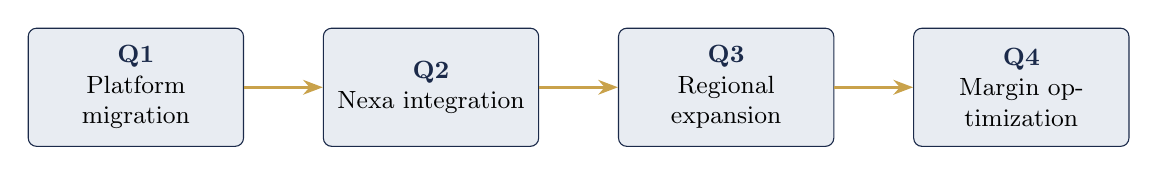
\begin{tikzpicture}[
  qbox/.style={draw=merinavy, fill=merilight, rounded corners=3pt, minimum width=2.7cm, minimum height=1.5cm, align=center, font=\small, text width=2.5cm},
]
\node[qbox] (q1) {\textbf{\textcolor{merinavy}{Q1}}\\Platform migration};
\node[qbox, right=1.0cm of q1] (q2) {\textbf{\textcolor{merinavy}{Q2}}\\Nexa integration};
\node[qbox, right=1.0cm of q2] (q3) {\textbf{\textcolor{merinavy}{Q3}}\\Regional expansion};
\node[qbox, right=1.0cm of q3] (q4) {\textbf{\textcolor{merinavy}{Q4}}\\Margin optimization};
\draw[-{Stealth[length=2.5mm]}, meringold, line width=1pt] (q1.east) -- (q2.west);
\draw[-{Stealth[length=2.5mm]}, meringold, line width=1pt] (q2.east) -- (q3.west);
\draw[-{Stealth[length=2.5mm]}, meringold, line width=1pt] (q3.east) -- (q4.west);
\end{tikzpicture}
}%
\end{center}
\vspace{0.5cm}
\begin{itemize}\small\setlength{\itemsep}{2pt}
  \item \textbf{Q1--Q2:} technical foundation and the Nexa partnership go live.
  \item \textbf{Q3--Q4:} commercial expansion converts into measurable margin gains.
\end{itemize}
\end{slide}

\sectiondivider{SECTION 03}{Financial Outlook}

\begin{slide}{Financial Highlights}
\begin{center}
\renewcommand{\arraystretch}{1.25}
\begin{tabular}{@{}lccc@{}}
\toprule
\rowcolor{merilight}
\textbf{Metric} & \textbf{FY2025A} & \textbf{FY2026E} & \textbf{FY2027E} \\
\midrule
Revenue (\$M) & 104 & 128 & 159 \\
EBITDA margin & 21\% & 24\% & 27\% \\
Free cash flow (\$M) & 18 & 27 & 41 \\
Net debt / EBITDA & 1.4x & 1.1x & 0.7x \\
\bottomrule
\end{tabular}
\end{center}
\vspace{0.4cm}
\begin{minipage}[t]{0.48\linewidth}
\begin{tcolorbox}[statbox]
\centering{\color{merinavy}\Large\textbf{\$159M}}\\
{\small\textcolor{merislate}{Projected FY2027E revenue}}
\end{tcolorbox}
\end{minipage}\hfill
\begin{minipage}[t]{0.48\linewidth}
\begin{tcolorbox}[statbox]
\centering{\color{merinavy}\Large\textbf{27\%}}\\
{\small\textcolor{merislate}{Target FY2027E EBITDA margin}}
\end{tcolorbox}
\end{minipage}
\end{slide}

\begin{slide}{Revenue Growth Trajectory}
\begin{center}
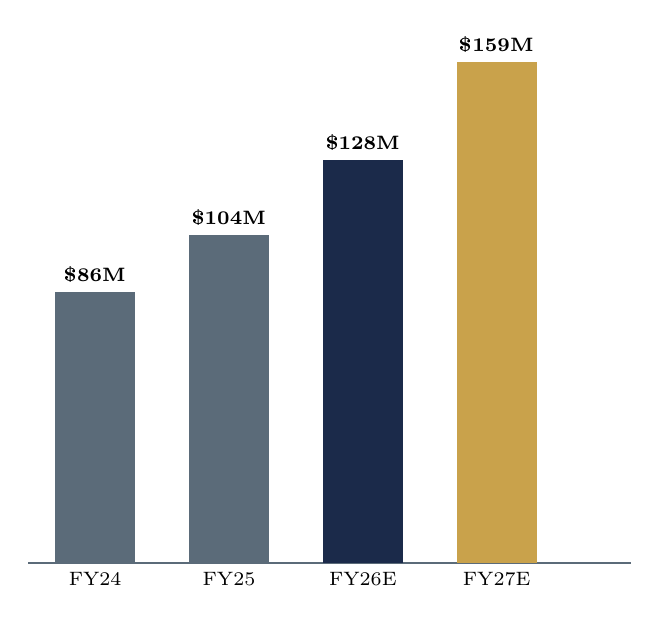
\begin{tikzpicture}[x=1.7cm,y=0.04cm]
\draw[merislate] (0,0) -- (4.5,0);
\foreach \x/\yr/\val/\lbl/\col in {%
  0.5/FY24/86/{\$86M}/merislate,%
  1.5/FY25/104/{\$104M}/merislate,%
  2.5/FY26E/128/{\$128M}/merinavy,%
  3.5/FY27E/159/{\$159M}/meringold%
}{
  \draw[fill=\col, draw=none] (\x-0.3,0) rectangle (\x+0.3,\val);
  \node[above] at (\x,\val) {\scriptsize\textbf{\lbl}};
  \node[below] at (\x,0) {\scriptsize \yr};
}
\end{tikzpicture}
\end{center}
\vspace{0.4cm}
{\small\textcolor{merislate}{\faChartLine\ Compound growth of 22.7\% projected across the FY2024--FY2027E window, led by the Q3--Q4 regional expansion.}}
\end{slide}

\sectiondivider{SECTION 04}{Execution \& Governance}

\begin{slide}{Leadership \& Accountability}
\begin{center}
\renewcommand{\arraystretch}{1.25}
\begin{tabular}{@{}lll@{}}
\toprule
\rowcolor{merilight}
\textbf{Pillar} & \textbf{Executive Owner} & \textbf{Function} \\
\midrule
Growth & Marcus Delgado & Chief Revenue Officer \\
Efficiency & Priya Anand & Chief Operating Officer \\
Resilience & Elena Whitfield & Chief Strategy Officer \\
Digital platform & Tomasz Kowalski & Chief Technology Officer \\
\bottomrule
\end{tabular}
\end{center}
\vspace{0.4cm}
\begin{itemize}
  \item \faCalendar\ Progress is reviewed at monthly steering committee meetings and reported to the Board quarterly.
  \item \faUsers\ Each pillar owner maintains a cross-functional working group with named deputies.
\end{itemize}
\end{slide}

\begin{slide}{Key Risks \& Mitigations}
\begin{center}
\renewcommand{\arraystretch}{1.3}
\begin{tabularx}{\linewidth}{@{}Xllc@{}}
\toprule
\rowcolor{merilight}
\textbf{Risk} & \textbf{Impact} & \textbf{Mitigation} & \textbf{Owner} \\
\midrule
Currency volatility across 42 markets & High & Natural hedging & Treasury \\
Talent attrition in platform engineering & Medium & Retention refresh & CTO \\
Client concentration in top 10 accounts & Medium & Pipeline diversification & CRO \\
Regulatory shifts in data residency & High & Regional data centers & Legal \\
\bottomrule
\end{tabularx}
\end{center}
\vspace{0.4cm}
{\small\textcolor{merislate}{\faFile\ Full risk register maintained by the Strategy Office; reviewed jointly with Legal \& Compliance each quarter.}}
\end{slide}

\begin{slide}{}
\vspace{1.3cm}
\begin{center}
{\huge\textbf{\textcolor{merinavy}{Thank You}}}\\[0.5cm]
{\color{meringold}\rule{4.2cm}{1.6pt}}\\[0.6cm]
{\large\textcolor{merislate}{Questions \& Discussion}}
\vspace{1.0cm}

\begin{tcolorbox}[statbox, width=0.7\linewidth]
\centering
\faUser\ \textbf{Elena Whitfield}, Chief Strategy Officer\\[4pt]
\faEnvelope\ strategy@meridiangroup.example\\[2pt]
\faPhone\ +1 (555) 019-4472\\[2pt]
\faGlobe\ www.meridiangroup.example
\end{tcolorbox}
\end{center}
\end{slide}

\end{document}
